\documentclass[aspectratio=169]{beamer}
\usepackage[utf8]{inputenc}
\usepackage{hyperref}
\usepackage{amsmath,amsfonts,amsthm,bm}
\usepackage{color}
\usepackage{minted}
\usepackage{graphicx} % Allows including images
\usepackage{booktabs} % Allows the use of \toprule, \midrule and \bottomrule in tables
\usepackage{tikz}
\usepackage[version=3]{mhchem}
\usepackage{pgfplots}
\pgfplotsset{compat=1.16} 
\setminted{fontsize=\scriptsize}


\hypersetup{
    colorlinks=true,
    linkcolor=red,
    filecolor=magenta,      
    urlcolor=red,
}

\DeclareMathOperator*{\argmax}{argmax}
\DeclareMathOperator*{\argmin}{argmin}
\let \vec \mathbf

\newcommand{\classname}{NANOx81}
\newcommand{\classyear}{Fall 2022}
\mode<presentation> {
    \usetheme{CambridgeUS}
    \setbeamertemplate{footline}[text line]{%
      \parbox{\linewidth}{\vspace*{-8pt}\classname\hfill\classyear\hfill\insertpagenumber}}

    %\setbeamertemplate{footline}[page number]
    \setbeamertemplate{navigation symbols}{}
}


\title[Python for Data Science and Materials Science]{Python for Data Science and Materials Science}

\author{Shyue Ping Ong}
\institute[UCSD]{University of California, San Diego\\
\medskip
}
\date{\classyear} % Date, can be changed to a custom date

\begin{document}


\begin{frame}
    \titlepage % Print the title page as the first slide
\end{frame}


\begin{frame}{Overview}
    \tableofcontents
\end{frame}


\section{Preliminaries}

\begin{frame}{Preliminaries}
    \begin{itemize}
        \item In this lecture, we will provide a brief overview of the Python programming language for data science and materials science.
        \item This will form the basis for your first lab on materials data wrangling in Python.
        \item Very quick overview of chapters 1-4 of the Python Data Science Handbook\cite{vanderplasPythonDataScience2016} + materials science libraries.
        \item Content is targeted at giving a complete beginner to Python and the scientific python stack enough background to get started.
        \item This lecture is extremely heavy on practical demos and examples. Please bring your laptop so that you can follow along.
        \item \textit{Coding is best learned by attempting to solve a practical problem.} The goal of this lecture is not to comprehensively cover all the libraries (which would be impossible in a one-quarter course).
    \end{itemize}
\end{frame}


\section{Python}

\begin{frame}{Python}
    \Huge{\centerline{Python}}
\end{frame} 

\begin{frame}{Introduction to Python}
    \centering{
\includegraphics[width=0.3\textwidth]{figures/python-logo.png}}
    \begin{itemize}
        \item General-purpose, high-level programming language
        \item Design emphasizes code readability
        \item Supports multiple programming paradigms (OOP, imperative, functional, procedural)
        \item Dynamically typed, automatic memory management and large standard library
        \item Available on almost all platforms
    \end{itemize}
    
\end{frame}


\begin{frame}[fragile]{Python vs other languages}
\begin{itemize}
    \item Java
    \inputminted{java}{example_hello_world_java.java}
    \item Python
    \inputminted{python}{example_hello_world_python.py}
\end{itemize}
\end{frame}

\begin{frame}{Python 3 or 2?}
    \begin{itemize}
        \item We will be using Python 3.8/3.9+.
        \item Modern version of Python that has been around since 2008 and is now the de facto standard from Jan 1 2020 - most major software packages are stopping support for Python 2 henceforth.
        \item Options for this course:
        \begin{itemize}
            \item Install python on your laptop - faster, not-reliant on internet connection, most modern version of Python possible.
            \item \href{https://colab.research.google.com/}{Google Colab} - Online Python notebooks. No installation required. But Python version and installed libraries lag the latest versions (sometimes by years). 
        \end{itemize}
    \end{itemize}
\end{frame} 


\begin{frame}{Installing Python}
    \begin{itemize}
        \item Regardless of whether your OS comes with Python, it is recommended that you install your own version of python using the Anaconda distribution.
        \item Two versions:
        \begin{description}
        \item[Miniconda] Minimal installation of Python interpreter itself + conda command-line tool. conda is essentially a package manager. \href{https://docs.conda.io/en/latest/miniconda.html}{Link}
        \item[Anaconda] Miniconda + several scientific packages such as scipy, numpy, etc. Several GB in size. \href{https://www.anaconda.com/distribution/}{Link}
        \end{description}
        \item Recommendation: Use miniconda to keep bloat to a minimum.
    \end{itemize}
\end{frame} 


\begin{frame}[fragile]{Basics of Python}
    \begin{itemize}
        \item Dynamically typed, i.e., no need for variable declaration.
        \inputminted{python}{example_basic_python.py}
        \item Other than some basic operations and functions, most other functions are in packages and modules and must be \textit{imported} prior to use.
        \inputminted{python}{example_imports.py}
        \item Please go through \href{https://docs.python.org/3/tutorial/index.html}{official Python tutorial}.
    \end{itemize}
\end{frame} 


\begin{frame}[fragile]{Virtual environments}
    \begin{itemize}
        \item Isolated environment for Python projects, i.e., each env has its own Python and packages.
        \item Both conda and python3 itself comes with the ability to create virtual environments.
        \begin{verbatim}
conda create --name nanox81 python=3.9
conda activate \classname
        \end{verbatim}
        \item To start over, you can remove the environment:
        \begin{verbatim}
conda remove --name nanox81 --all
        \end{verbatim}
        \item You can also create reproducible environments from a file.
        \begin{verbatim}
conda env create -f nanox81_env.yml
        \end{verbatim}
        \item Example nanox81\_env.yml file given in the \href{https://github.com/materialsvirtuallab/\classname}{\classname Github repo}.
    \end{itemize}
\end{frame}


\begin{frame}[fragile]{Installing packages using conda}
    \begin{itemize}
        \item We will get into the details of the specific packages later.
    \begin{verbatim}
# Scientific python stack
conda install numpy scipy matplotlib seaborn jupyter
# Data Science tools
conda install pandas scikit-learn tensorflow
# Materials science library
conda install --channel conda-forge pymatgen
    \end{verbatim}
        \item To update a package, use:
    \begin{verbatim}
conda update numpy
    \end{verbatim}
    \end{itemize}
\end{frame}


\begin{frame}[fragile]{Google Colab Demo}
    \begin{itemize}
        \item URL: \url{https://colab.research.google.com}
        \item Start a new blank notebook or download one from Github.
        \begin{figure}
            \centering
            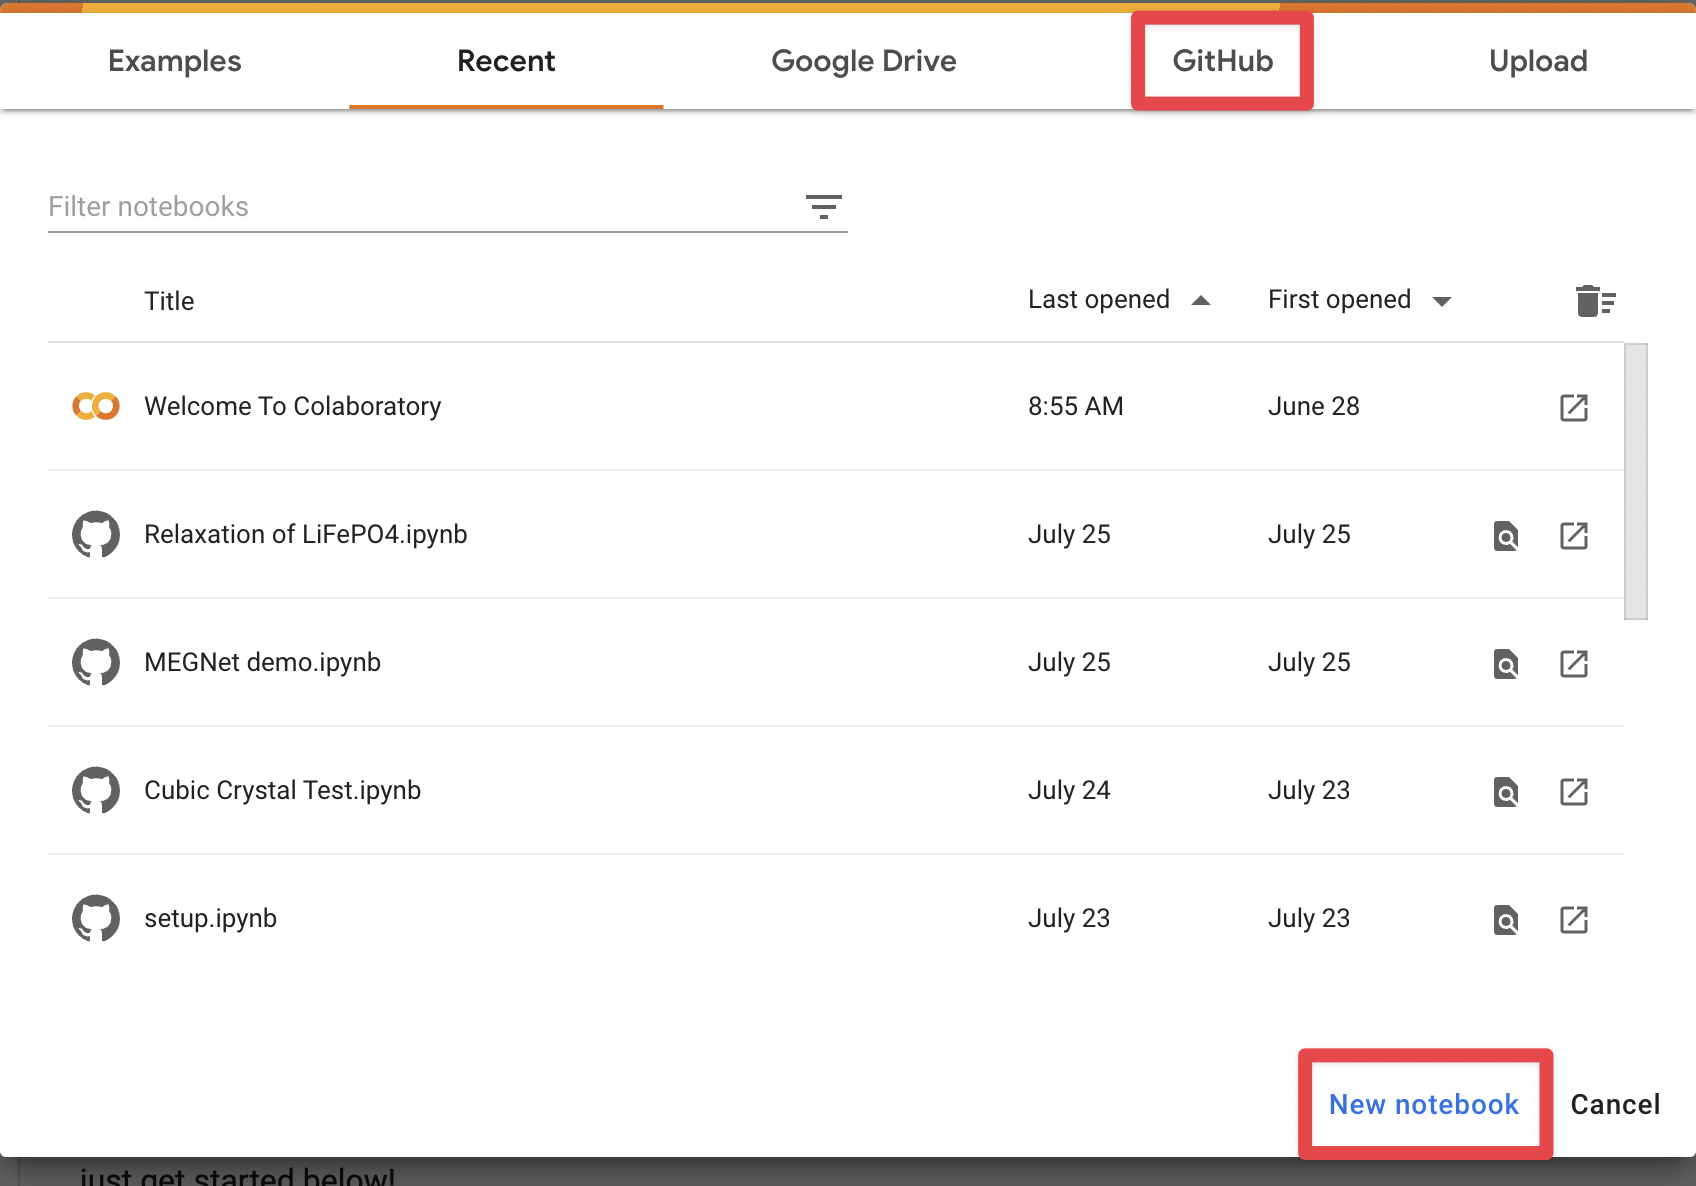
\includegraphics[height=0.25\textwidth]{lectures/slides_tex/figures/GoogleColab.png}
            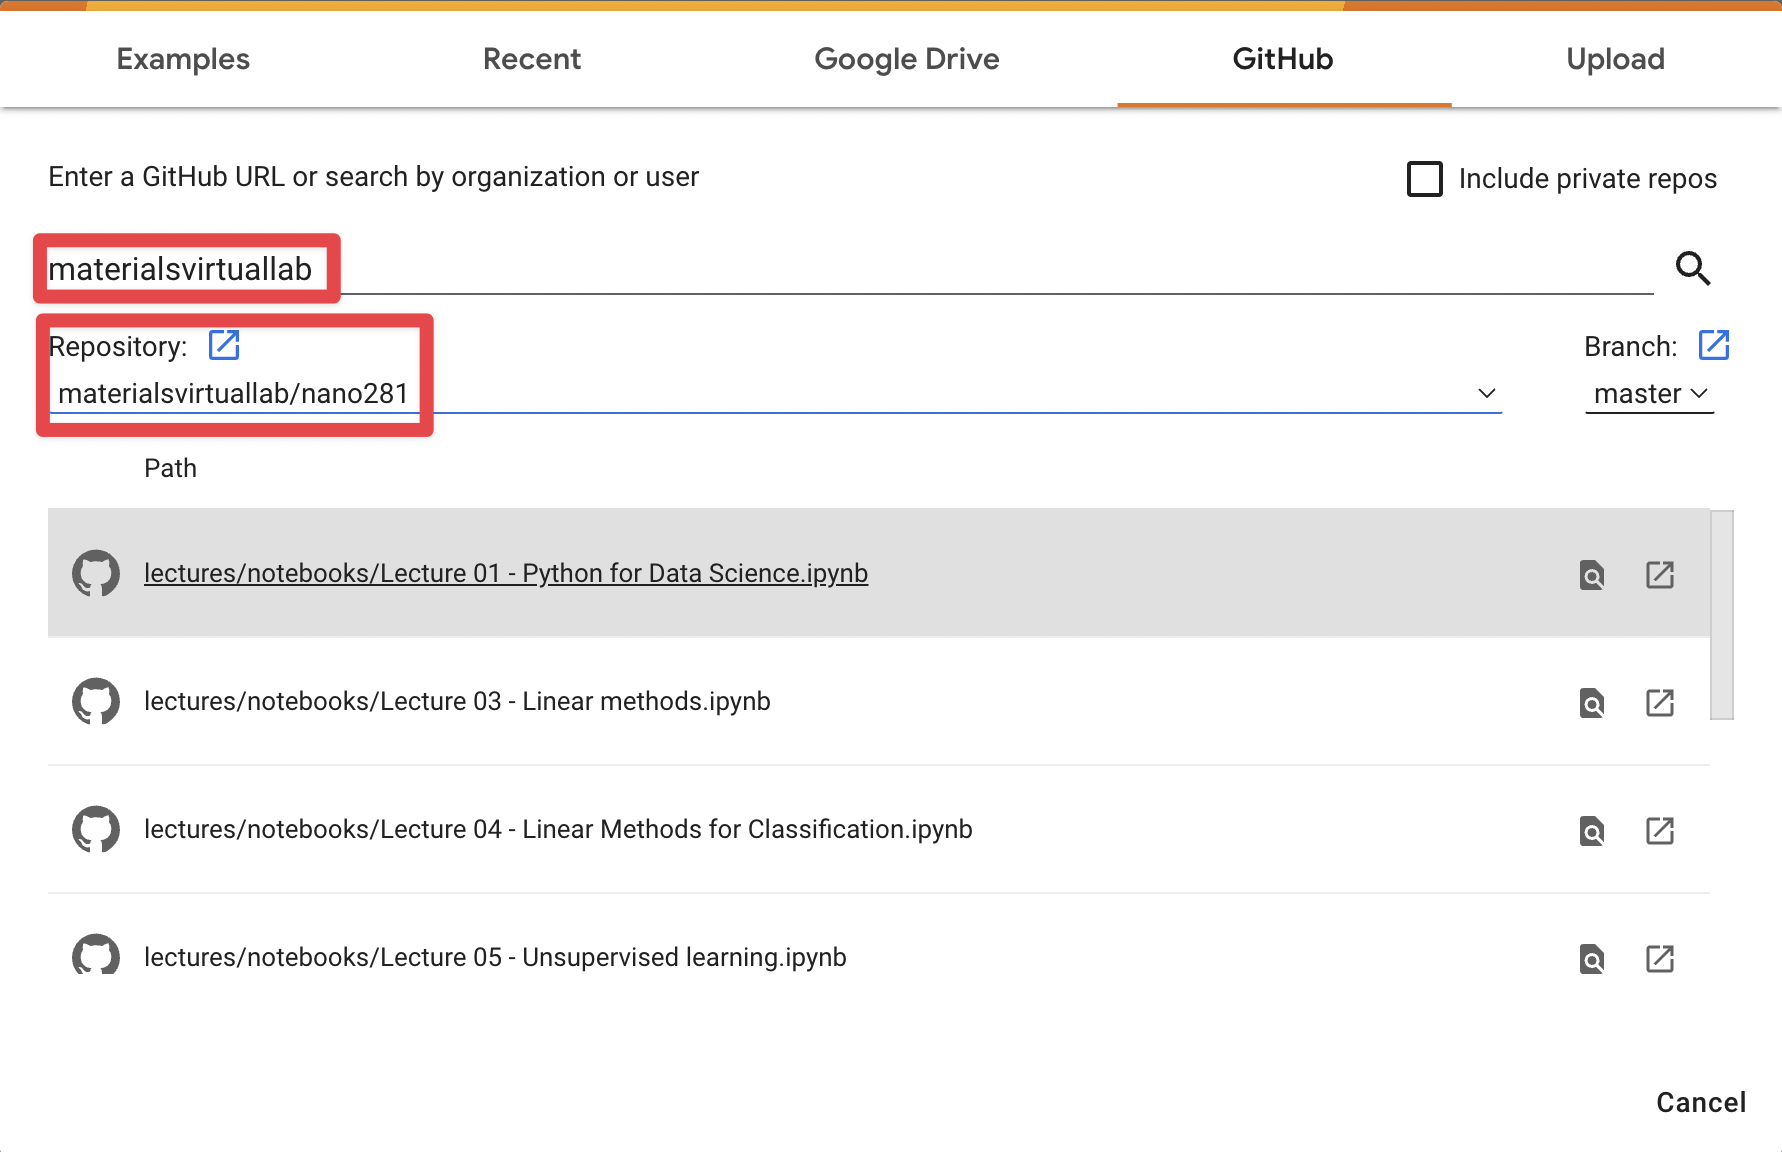
\includegraphics[height=0.25\textwidth]{lectures/slides_tex/figures/GoogleColabGithub.png}
        \end{figure}
        \item Most of the data science packages we will be using in this course are pre-installed.
        \item To install a missing package (e.g., pymatgen), add the following in the first cell:
\begin{verbatim}
    ! pip install pymatgen
\end{verbatim}        
    \end{itemize}
\end{frame}




\section{Scientific python stack}

\begin{frame}{Scientific Python}
    \Huge{\centerline{Scientific Python}}
\end{frame} 

\begin{frame}{Scientific Python Packages}
\begin{figure}
    \centering
    
\includegraphics[height=0.7cm]{figures/jupyter-logo.png}
    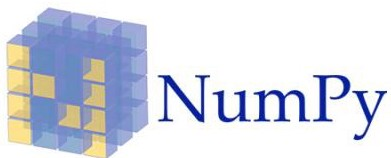
\includegraphics[height=0.7cm]{figures/numpy-logo.jpeg}
    
\includegraphics[height=0.7cm]{figures/scipy-logo.png}
    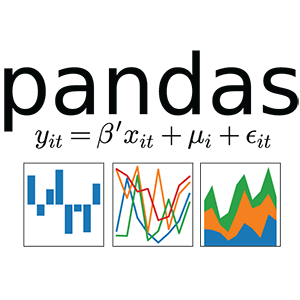
\includegraphics[height=0.7cm]{figures/pandas-logo.png}
    
\includegraphics[height=0.7cm]{figures/scikit-learn-logo.png}
    
\includegraphics[height=0.7cm]{figures/tensorflow-logo.png}
\end{figure}
    \begin{description}
        \item[\href{http://jupyter.org/}{jupyter}] Software for interactive computing
        \item[\href{http://www.scipy.org/}{Numpy}] Fundamental package for numerical computation. Defines array and matrix types and basic operations on them.
        \item[\href{http://www.scipy.org/}{Scipy}] Efficient numerical routines such as routines for numerical integration and optimization.
        \item[\href{http://pandas.pydata.org/}{pandas}] High-performance, easy to use data structures.
        \item[\href{http://scikit-learn.org/}{scikit-learn}] Tools for predictive data analysis.
        \item[\href{http://www.tensorflow.org/}{TensorFlow}] Library for developing and training ML models.
        \item[\href{http://matplotlib.org/}{matplotlib}] De facto plotting library
        \item[\href{http://seaborn.pydata.org/}{seaborn}] Statistical data visualization
    \end{description}
\end{frame}


\begin{frame}{Brief note on coverage}
    \begin{itemize}
        \item In the following slides, we will provide a brief background on all these packages, with a heavy focus on actual demos.
        \item It should be noted that most of these packages have an extensive suite of functionality and it is not possible to comprehensively go through them in this course. 
        \item Focus will be on modules and methods that pertain to the data science problem we are solving. You are expected to learn to navigate the relevant documentation pages of each package (plus a generous amount of googling) to identify the appropriate module or method for what you need to do.
        \item numpy and scipy are the backbone for many of the other packages such as pandas and scikit-learn. You need to ensure you understand the basics of numpy arrays and how to perform various simple linear algebra operations. In most instances, the actual data science package (scikit-learn) will be the one you interact with most.
    \end{itemize}
\end{frame} 


\begin{frame}[fragile]{Jupyter notebook}
    \begin{itemize}
        \item We will primarily be using Jupyter for its notebook application, though it is capable of a lot more. (Google Colab is similar.)
        \item Jupyter Notebook is an open-source web application to create and share documents that contain code, equations, visualizations and narrative text, etc.
        \item All lecture examples will be done in Jupyter notebooks. You will also be submitting notebooks (ipynb files) as your lab reports.
        \item Document: \href{http://jupyter-notebook.readthedocs.io/en/stable/}{link}
        \item Running a jupyter notebook:
        \begin{verbatim}
        jupyter notebook
        \end{verbatim}
        \item The notebook server will be running at http://localhost:8888 (typically).
    \end{itemize}
\end{frame}


\begin{frame}{Jupyter notebook, contd.}
    \begin{itemize}
        \item Things you can do in a notebook:
        \begin{itemize}
            \item Run code in a cell with `shift+return` - helpful things include tab completion, magic functions (e.g., ?, ! and \% are the key ones to know, especially ?).
            \item Write text/narrative - set cell to markdown mode and write markdown.
            \item Make plots (highly recommend that you put ``\%matplotlib inline'' near the start of your notebook to display graphs inline).
        \end{itemize}
        \item Very useful for quick code prototyping and data analysis.
    \end{itemize}
\end{frame}


\begin{frame}{Numpy}
    \begin{itemize}
        \item Implements the array and matrix objects.
        \item Underlying implementation is in C, and hence extremely efficient.
        \item Vectorization of operations, as opposed to loops, is key to efficiency.
        \item Recommend that you focus on the array object and ignore the matrix object.
        \item Note that standard operations such as +, -, * and / for np.arrays are element-wise. For matrix multiplications, use special numpy functions, e.g., numpy.dot or the new @ operator available in Python 3.7 and above.
        \item For those of you who are familiar with Matlab, it helps to read the \href{https://docs.scipy.org/doc/numpy/user/numpy-for-matlab-users.html}{Numpy for Matlab users doc}.
        \item Documentation: \href{http://docs.scipy.org/doc/numpy/}{link}
    \end{itemize}
\end{frame}


\begin{frame}[fragile]{Numpy examples}
    \inputminted{python}{example_numpy.py}
\end{frame}


\begin{frame}[fragile]{Scipy}
    \begin{itemize}
        \item Efficient numerical routines for numerical integration, interpolation, optimization, linear algebra, and statistics, etc.
        \item scipy.linalg is a superset of numpy.linalg, and is always compiled with BLAS/LAPACK. So use scipy.linalg.
        \item Dependency for most other packages you will be using.
    \inputminted{python}{example_scipy.py}
    \item Documentation: \href{https://docs.scipy.org/doc/scipy/reference/}{link}
    \item Scipy lectures (very useful resource): \href{https://scipy-lectures.org/}{link}
    \end{itemize}
\end{frame}


\begin{frame}{Pandas}
    \begin{itemize}
        \item Data analysis library
        \item Data structures designed for working with relational or labeled data
        \item Two main data types:
        \begin{description}
        \item[Series] 1D labeled homogeneously-typed array
        \item[DataFrame] 2D labeled, size-mutable tabular structure with potentially heterogeneously-typed column
        \end{description}
        \item It is helpful to think of DataFrame as essentially a Python object representing the contents of a table, e.g. such as what you would have in Excel spreadsheet. This is similar to the dataframe in R.
        \item Please go through the \href{http://pandas.pydata.org/pandas-docs/stable/getting_started/10min.html}{10 minute guide to pandas}.
    \end{itemize}
\end{frame}


\begin{frame}[fragile]{Pandas demo}
    \begin{itemize}
        \item For this demo, we will utilize data that has been published by the MAterials Simulation Toolkit - Machine Learning (MAST-ML) on figshare.
    \end{itemize}
\inputminted{python}{example_pandas.py}
\end{frame}


\begin{frame}{scikit-learn \& TensorFlow}
    \begin{itemize}
        \item Packages for machine learning.
        \item To some extent, scikit-learn and TensorFlow (TF) overlap in functionality.
        \item For the purposes of this course, we will use mainly scikit-learn for ML and will briefly touch on TF for neural networks.
        \item We will defer all specific code examples for scikit-learn and TF until we go through specific types of ML models, e.g., linear regression, kernel regression, etc. Having the theory background of the ML methods will make it easier to understand the code usage and implementations.
        \item Instead, we will provide an overview of the high-level API design of scikit-learn.
    \end{itemize}
\end{frame} 


\begin{frame}[fragile]{Scikit-learn Model API}
    \begin{itemize}
        \item All ML models inherit from BaseEstimator and various mix-in classes with standardized method names.
        \inputminted{python}{example_sklearn.py}
        \item Note that the params and score depends on the specifics of the ML model type.
    \end{itemize}
\end{frame} 



\begin{frame}[fragile]{Matplotlib and Seaborn}
    \begin{itemize}
        \item Plotting libraries.
        \item Matplotlib is the de facto library for generating all kinds of plots and many other plotting engines (including seaborn) are built on top of it
        \item seaborn is a extremely helpful package for statistical data visualization. Works very well with Pandas DataFrame.
\inputminted{python}{example_plotting.py}
        \item \href{http://seaborn.pydata.org/examples/index.html}{Seaborn gallery} contains may visual examples with source code. 
    \end{itemize}
\end{frame} 


\section{Materials analysis}

\begin{frame}{Materials Analysis}
    \Huge{\centerline{Materials Analysis}}
\end{frame} 

\begin{frame}{Python Materials Genomics (pymatgen)}
    \begin{itemize}
        \item Core materials analysis powering the Materials Project.\cite{ongPythonMaterialsGenomics2013}
        \item Defines core extensible Python objects for materials data representation.
        \item Provides a robust and well-documented set of structure and thermodynamic analysis tools relevant to many applications.
        \item Establishes an open platform for researchers to collaboratively develop sophisticated analyses of materials data.
        \item High-level methods to access the Materials Project API.\cite{ongMaterialsApplicationProgramming2015} (particularly useful for this course).
    \end{itemize}
\end{frame}


\begin{frame}{Overview of capabilities}
    \begin{figure}
        \centering
        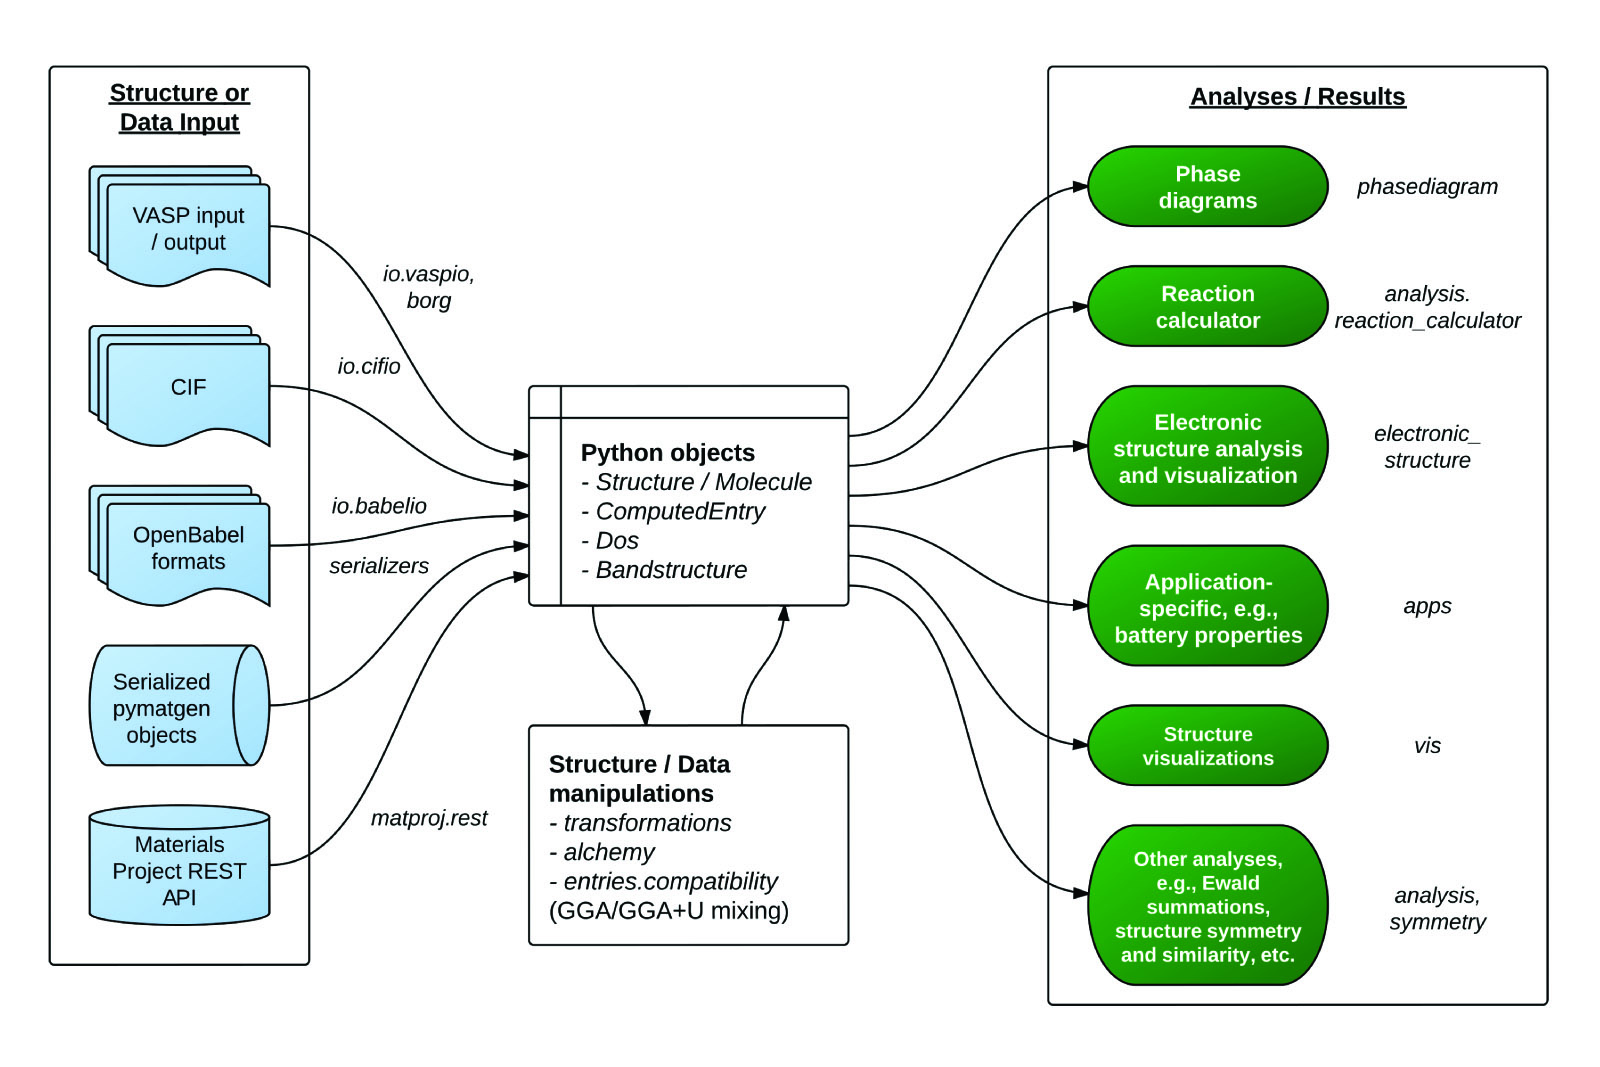
\includegraphics[width=0.6\textwidth]{figures/pymatgen-overview.jpg}
    \end{figure}
\end{frame}


\begin{frame}[fragile]{Accessing the Materials API}
    \begin{itemize}
        \item Accessed using the pymatgen.ext.matproj.MPRester class.
        \item While there are many convenience methods to query for crystal structures and other object types, the most powerful and useful method for data analysis is the MPRester's query method.
        \item This method has to be used in conjunction with the Materials API documentation available at \url{https://github.com/materialsproject/mapidoc}.
\inputminted{python}{example_materials_api.py}
    \end{itemize}
\end{frame} 


\begin{frame}[allowframebreaks]{Bibliography}
    \bibliographystyle{unsrt}
    \bibliography{refs}
\end{frame}


\begin{frame}
    \Huge{\centerline{The End}}
\end{frame}

\end{document}

